\documentclass[../../main]{subfiles}

\begin{document}
\chapter{ヒルベルト空間}
\label{chapter:hilbert_space}

\section{イントロダクション}

\begin{figure}[htbp]
  \centering
  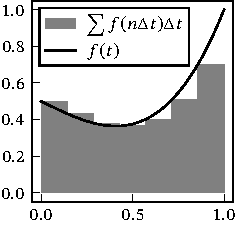
\includegraphics{figures/riemann_sum.pdf}
  \caption{\(f(t)\)と\(\sum f(n\increment t)\increment t\)の比較.}
\end{figure}

\[
  \sum_{n=0}^{N-1}x(n\increment t)\conj*{y(n\increment t)}\increment t \to \int_0^1x(t)\conj*{y(t)}\intd{t}\quad(N\to\infty)
\]

\pagebreak

\section{無限次元のベクトル空間}

\subsection{距離空間}

\begin{definition}{距離}{metric}\index{きょり@距離}
  \(S\)を集合とする.\(d\)が\(S\)上の\termdef{距離}(metric)であるとは,
  任意の\(x,y,z\in S\)に対して,\(d\)が以下の条件を満たすことをいう.
  \begin{enumerate}
    \item \(d(x,y)\geq 0\),\([d(x,y)=0\iff x=y]\)
    \item \(d(x,y)=d(y,x)\)
    \item \(d(x,y)+d(y,z)\geq d(x,z)\)
  \end{enumerate}
\end{definition}

集合と距離の組\((S,d)\)を\termdef{距離空間}\index{きょりくうかん@距離空間}(metric space)という.

\begin{example}
  \label{example:metric_space}
  \(S=\numset{C}\),\(d(z,w)=\abs{z-w}\)とすると,\((S,d)\)は距離空間になる.
\end{example}

\begin{example}[離散距離]
  \label{example:discrete_metric}
  集合\(S\)は空でないとする.また,各\(x,y\in S\)に対して,\(x=y\)のとき\(d(x,y)=0\),\(x\neq y\)のとき\(d(x,y)=1\)とする.
  このとき\(d\)は\(S\)上の距離になる.距離\(d\)を\termdef{離散距離}\index{りさんきょり@離散距離}(discrete metric),
  距離空間\((S,d)\)を\termdef{離散空間}\index{りさんくうかん@離散空間}(discrete space)という.
\end{example}

\cref{definition:metric}のように抽象的な形で距離を定義する利点の1つは,\(\numset{K}^n\)以外の集合に対しても,点列の極限を定義できることである.

\begin{definition}{点列の収束}{sequence_converge}\index{しゅうそくてんれつの@収束,点列の}
  \((S,d)\)を距離空間とする.\(S\)上の点列\(\seq{x_n}_{n\in\numset{N}}\)が\(\alpha\in S\)に\termdef{収束する}(converge)とは,
  任意の\(\varepsilon>0\)に対し,\(N\in\numset{N}\)が存在して\(n>N\implies d(x_n,\alpha)<\varepsilon\)を満たすことをいう.
  このことを次のように表す.
  \[
    x_n\to\alpha\quad(n\to\infty)
  \]
\end{definition}

\begin{note}
  次の命題が成り立つことに注意.
  \[
    x_n \to \alpha\quad(n\to\infty)
    \iff\lim_{n\to\infty}d(x_n,\alpha) = 0
  \]
\end{note}

\(\seq{x_n}_{n\in\numset{N}}\)が\(\alpha\)に収束するとき,\(\alpha\)を\(\seq{x_n}_{n\in\numset{N}}\)の\termdef{極限点}\index{きょくげんてん@極限点}(limit point)という.
\cref{definition:sequence_converge}は要するに「\(N\)の値を十分に大きくとれば,点\(x_{N+1},x_{N+2},\dotsc\)が点\(\alpha\)から距離\(\varepsilon\)以上離れないようにできる」ことを意味する.

\begin{example}
  \label{example:complex_planes_convergence}
  \((S,d)\)を\cref{example:metric_space}の距離空間とする.\(S\)上の点列\(\seq{z_n}_{n\in\numset{N}}\)を\(z_n=(\sqrt{3}+\iuni)/(2n)\)で定義すると,
  \(\seq{z_n}_{n\in\numset{N}}\)は\cref{definition:sequence_converge}の意味で\(z_n\to 0\)(\(n\to\infty\))を満たす.
\end{example}

\begin{example}[一様収束]
  \label{example:uniform_converge}
  閉区間\(I\)は有界とする.連続関数\(f\colon I\to\numset{R}\)の全体集合を\(\cont{0}(I)\)とおくと,\(d(f,g)=\max\Set{\abs{f(t)-g(t)}\given x\in I}\)は\(\cont{0}(I)\)上の距離になる.
  \(\cont{0}(I)\)上の関数列\(\seq{f_n}_{n\in\numset{N}}\)が\cref{definition:sequence_converge}の意味で\(f\in\cont{0}(I)\)に収束するとき,
  \(\seq{f_n}_{n\in\numset{N}}\)は\(f\)に\termdef{一様収束する}\index{いちようしゅうそく@一様収束}(converge uniformly)という.

  たとえば\(I=[0,1]\),\(f_n(t)=(1/n)\abs{\sin(n\krez t)}\)のとき,\(\seq{f_n}_{n\in\numset{N}}\)は定数関数\(\phi(t)=0\)に一様収束する.
  実際\(d(f_n,\phi)=\max\Set{\abs{f_n(t)}\given t\in I}=1/n\)なので,\(n\)の値を十分大きくとれば\(d(f_n,\phi)\)の値を限りなく小さくできる(\cref{figure:uniform_converge}).
\end{example}

\begin{figure}[htbp]
  \begin{minipage}{0.5\linewidth}
    \centering
    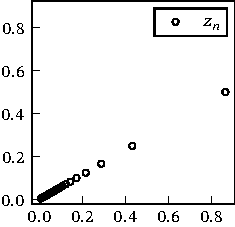
\includegraphics{figures/complex_convergence.pdf}
    \caption{\(z_n\to 0\)(\(n\to\infty\))の様子.}
    \label{figure:sequence_converge}
  \end{minipage}%
  \begin{minipage}{0.5\linewidth}
    \centering
    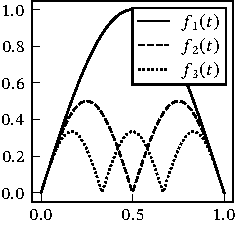
\includegraphics{figures/func_convergence.pdf}
    \caption{\(f_n\to\phi\)(\(n\to\infty\))の様子.}
    \label{figure:uniform_converge}
  \end{minipage}
\end{figure}

\begin{note}
  \cref{example:complex_planes_convergence}において\(\abs{z_n}=1/n\)であるから,\(d(f_n,\phi)=\abs{z_n}\)である.
  よって,\cref{figure:sequence_converge}は(\(z_n\)を\(f_n\)に書き換えれば)\(f_n\to\phi\)(\(n\to\infty\))の様子を描いた図とも考えられる.
  このように,関数などの一見「点」とは思えないような対象を点とみなして考察するのは,しばしば理解の助けになる.
\end{note}

\begin{proposition}{}{limit_uniqueness}
  極限点は存在すれば一意である.すなわち,距離空間\((S,d)\)上の点列\(\seq{x_n}_{n\in\numset{N}}\)が\(\alpha,\beta\in S\)に収束するなら,\(\alpha=\beta\)である.
\end{proposition}

\begin{proof}
  \(0\leq d(\alpha,\beta)\leq d(\alpha,x_n)+d(x_n,\beta)=d(x_n,\alpha)+d(x_n,\beta)\)なので,\(d(x_n,\alpha)\to 0\),\(d(x_n,\beta)\to 0\)(\(n\to\infty\))なら\(d(\alpha,\beta)=0\),\(\alpha=\beta\)である.
\end{proof}

\cref{proposition:limit_uniqueness}から,各収束列\(\seq{x_n}_{n\in\numset{N}}\)に対して,その極限点は一意に定まる.そのため,以降は収束列\(\seq{x_n}_{n\in\numset{N}}\)の極限点を
\[
  \lim_{n\to\infty}x_n
\]
と書く.

\begin{definition}{閉包・閉集合・稠密}{closure}\index{へいほう@閉包}\index{へいしゅうごう@閉集合}\index{ちゅうみつ@稠密}\index{cl@\(\clsr S\)}
  \((S,d)\)を距離空間,\(A\)を\(S\)の部分集合とする.
  \begin{enumerate}
    \item \(A\)上の収束列すべての極限点からなる集合を\(A\)の\termdef{閉包}(closure)といい,\(\clsr A\)と書く\footnotemark .
    \item \(A=\clsr A\)であるとき,\(A\)は\termdef{閉集合}(closed set)であるという.
    \item 集合\(B\subset A\)が\(\clsr B=A\)を満たすとき,\(B\)は\(A\)において\termdef{\ltjruby{稠密}{ちゆうみつ}}(dense)であるという.
  \end{enumerate}
\end{definition}

\footnotetext{本書では閉包を\(\clsr A\),補集合を\(\scomp{A}\)\index{c@\(\scomp{S}\)}で表す.}

\begin{example}
  \(\clsr\ocival{0}{1}=\ccival{0}{1}\),\(\clsr\numset{Q}=\numset{R}\)である.
\end{example}

\begin{definition}{コーシー列}{cauchy_sequence}\index{こーしーれつ@コーシー列}
  \((S,d)\)を距離空間とする.\(S\)上の点列\(\seq{x_n}_{n\in\numset{N}}\)が\termdef{コーシー列}(Cauchy sequence)であるとは,
  任意の\(\varepsilon>0\)に対し,\(N\in\numset{N}\)が存在して\(m,n>N\implies d(x_m,x_n)<\varepsilon\)を満たすことをいう.このことを次のように表す.
  \[
    d(x_m,x_n) \to 0\quad(m,n\to\infty),
    \quad\lim_{m,n\to\infty}d(x_m,x_n) = 0
  \]
\end{definition}

また,\(S\)上の任意のコーシー列が収束列でもあるとき,\((S,d)\)は\termdef{完備距離空間}\index{かんびきょりくうかん@完備距離空間}\index{きょりくうかん@距離空間!かんび@完備\texttwoemdash}(complete metric space)であるという.
一般に収束列はコーシー列でもあるから,完備距離空間において収束列とコーシー列は同値な概念である.

\begin{example}
  \(S=\numset{Q}\),\(d(x,y)=\abs{x-y}\)とすると,\((S,d)\)は距離空間になるが完備距離空間にはならない.
\end{example}

\subsection{ノルム空間}

\begin{definition}{ノルム}{norm}\index{のるむ@ノルム}\indexsymbol{\(\vnorm{\holder}\)}
  \(V\)を\(\numset{K}\)上のベクトル空間とする.\(\vnorm{\holder}\)が\(V\)の\termdef{ノルム}(norm)であるとは,
  任意の\(\lambda\in\numset{K}\),\(x,y\in V\)に対して,\(\vnorm{\holder}\)が以下の条件を満たすことをいう.
  \begin{enumerate}
    \item \(\vnorm{x}\geq 0\),\([\vnorm{x}=0\iff x=0]\)
    \item \(\vnorm{\lambda x}=\abs{\lambda}\vnorm{x}\)
    \item \(\vnorm{x+y}\leq\vnorm{x}+\vnorm{y}\)
  \end{enumerate}
\end{definition}

ノルムが備わっているベクトル空間のことを\termdef{ノルム空間}\index{のるむくうかん@ノルム空間}(normed space)という.
\(V\)がノルム空間であれば,\(d(x,y)=\vnorm{x-y}\)(\(x,y\in V\))により\(V\)上の距離\(d\)が定義される.
\((V,d)\)が完備距離空間であるとき,\(V\)は\termdef{バナッハ空間}\index{ばなっはくうかん@バナッハ空間}(Banach space)であるという.

\begin{example}
  \(V\)が\(\numset{K}\)上の内積空間なら,\(V\)の内積\(\innerp{\holder}{\holder}\)から\(V\)のノルムを\(\vnorm{x}=\sqrt{\innerp{x}{x}}\)で定義できる.
  つまり,内積空間はノルム空間でもある.
\end{example}

\begin{example}[\(\lebesgue{p}\)空間]
  複素数列\(\seq{x_n}_{n\in\numset{N}}\)に対して,\(\vnorm{\seq{x_n}_{n\in\numset{N}}}_p\in\ccival{0}{+\infty}\)(\(p\geq 1\))を
  \[
    \lpnorm{p}{\seq{x_n}_{n\in\numset{N}}} = \pqty*{\sum_{n=1}^\infty\abs{x_n}^p}^{1/p}
  \]
  で定義する.\(\numset{C}^{\numset{N}}\)の部分空間\(\lebesgue{p}(\numset{N})\)を\(\lebesgue{p}(\numset{N})=\Set*{\seq{x_n}_{n\in\numset{N}}\given\lpnorm{p}{\seq{x_n}_{n\in\numset{N}}}<+\infty}\)
  で定義すると,\(\lpnorm{p}{\holder}\)は\(\lebesgue{p}\)のノルムになり,しかも,\(\lebesgue{p}(\numset{N})\)はこのノルムについてバナッハ空間になる.
  バナッハ空間\(\lebesgue{p}(\numset{N})\)を\termdef{\(\lebesgue{p}\)空間}\index{lpkukan@\(\lebesgue{p}\)空間}(\(\lebesgue{p}\) space)という.
\end{example}

\begin{example}
  \cref{example:uniform_converge}の集合\(\cont{0}(I)\)は,ノルム\(\vnorm{f}_\infty=\max\Set{\abs{f(t)}\given t\in I}\)についてバナッハ空間になる.
  ただし,関数の和\(\phi=f+g\)とスカラー倍\(\psi=\lambda f\)はそれぞれ\(\phi(t)=f(t)+g(t)\),\(\psi(t)=\lambda\cdot(f(t))\)で定義する.
\end{example}

\section{ヒルベルト空間}

\begin{definition}{ヒルベルト空間}{hilbert_space}\index{ひるべるとくうかん@ヒルベルト空間}
  内積空間\(H\)が\termdef{ヒルベルト空間}(Hilbert space)であるとは,
  \(H\)の内積\(\innerp{\holder}{\holder}\)から定まるノルム\(\vnorm{x}=\sqrt{\innerp{x}{x}}\)について,\(H\)がバナッハ空間であることをいう.
\end{definition}

もう少し定義をさかのぼると,ノルム空間\(H\)がバナッハ空間であるとは,距離\(d(x,y)=\vnorm{x-y}\)について\((H,d)\)が完備距離空間であることをいうのであった.
したがって,完備距離空間・ノルム空間・バナッハ空間・内積空間が有する性質はすべて,ヒルベルト空間にも引き継がれる.

\begin{note}
  以下に述べる命題は,内積空間であればすべて成立する.内積空間がヒルベルト空間であるための条件「完備性」は,条件を満たす点列に対して,極限点の存在を保証するものである.
  そのため,ヒルベルト空間でないと成立しない定理は,存在を主張する定理であることが多い.
  本書においても,存在定理である\cref{theorem:convex_projection_theorem}で初めて,完備性が本質的に効いてくる.
\end{note}

\begin{theorem}{中線定理}{median_theorem}\index{ちゅうせんていり@中線定理}
  \(V\)を内積空間とするとき,任意の\(x,y\in V\)に対して\(\vnorm{x+y}^2+\vnorm{x-y}^2=2(\vnorm{x}^2+\vnorm{y}^2)\)が成立する.
\end{theorem}

\begin{proof}
  実際\(\vnorm{x+y}^2+\vnorm{x-y}^2=(\vnorm{x}^2+2\rpart\innerp{x}{y}+\vnorm{y}^2)+(\vnorm{x}^2-2\rpart\innerp{x}{y}+\vnorm{y}^2)=2(\vnorm{x}^2+\vnorm{y}^2)\)である.
\end{proof}

\begin{theorem}{コーシー・シュワルツの不等式}{cauchy_schwarz}\index{こーしーしゅわるつのふとうしき@コーシー・シュワルツの不等式}
  \(V\)を内積空間とする.このとき,任意の\(a,b\in V\)について\(\abs{\innerp{a}{b}}\leq\vnorm{a}\vnorm{b}\)が成立する.
  これを\termdef{コーシー・シュワルツの不等式}(Cauchy–Schwarz inequality)という.
\end{theorem}

\begin{proof}
  \(b\neq 0\)のときについて示す.\(\lambda=\innerp{a}{b}/\vnorm{b}^2\),\(a_{\mathord{\perp}}=a-\lambda b\)とおくと,\(\innerp{a_{\mathord{\perp}}}{b}=0\)より
  \(
    \vnorm{a_{\mathord{\perp}}}^2 = \innerp{a_{\mathord{\perp}}}{a_{\mathord{\perp}}}
    = \innerp{a-\lambda b}{a_{\mathord{\perp}}}
    = \innerp{a}{a_{\mathord{\perp}}} - \lambda\innerp{b}{a_{\mathord{\perp}}}
    = \innerp{a}{a_{\mathord{\perp}}}
  \)
  である.よって
  \(
    \vnorm{a_{\mathord{\perp}}}^2 = \innerp{a}{a-\lambda b}
    = \vnorm{a}^2-\conj{\lambda}\innerp{a}{b}
    = \vnorm{a}^2-\abs{\innerp{a}{b}}^2/\vnorm{b}^2
  \)
  だから,\((\vnorm{a}\vnorm{b})^2-\abs{\innerp{a}{b}}^2=(\vnorm{a_{\mathord{\perp}}}\vnorm{b})^2\geq 0\)である.
\end{proof}

\begin{proposition}{ノルムの連続性}{norm_continuous}
  \(V\)がノルム空間なら,\(V\)上の任意の収束列\(\seq{x_n}\)について次式が成立する.
  \[
    \lim_{n\to\infty}\vnorm{x_n} = \vnorm*{\lim_{n\to\infty}x_n}
  \]
\end{proposition}

\begin{proof}
  \(\seq{x_n}\)を\(V\)上の収束列とし,極限点を\(a\)とおく.
  このとき\(\vnorm{x_n}\leq\vnorm{x_n-a}+\vnorm{a}\),\(\vnorm{a}\leq\vnorm{a-x_n}+\vnorm{x_n}\)なので
  \(\abs{\vnorm{x_n}-\vnorm{a}}\leq\vnorm{x_n-a}\to 0\)(\(n\to\infty\)),よって\(\vnorm{x_n}\to\vnorm{a}\)(\(n\to\infty\))である.
\end{proof}

\begin{proposition}{内積の連続性}{inner_products_continuous}
  \(V\)が内積空間なら,\(V\)上の任意の収束列\(\seq{x_n}\),\(\seq{y_n}\)について次式が成立する.
  \[
    \lim_{k\to\infty}\innerp{x_k}{y_k} = \innerp*{\lim_{m\to\infty}x_m}{\lim_{n\to\infty}y_n}
  \]
\end{proposition}

\begin{proof}
  \(x_n\to a\),\(y_n\to b\)(\(n\to\infty\))とする.
  \(\innerp{x_n}{y_n}=\innerp{x_n-a}{y_n}+\innerp{a}{y_n-b}+\innerp{a}{b}\)だから,
  \nameref{theorem:cauchy_schwarz}より\(\abs{\innerp{x_n}{y_n}-\innerp{a}{b}}\leq\abs{\innerp{x_n-a}{y_n}}+\abs{\innerp{a}{y_n-b}}\leq\vnorm{x_n-a}\vnorm{y_n}+\vnorm{a}\vnorm{y_n-b}\)である.
  \cref{proposition:norm_continuous}より\(\vnorm{x_n-a}\vnorm{y_n}\to 0\vnorm{b}\),\(\vnorm{y_n-a}\to 0\)(\(n\to\infty\))なので,\(\innerp{x_n}{y_n}\to\innerp{a}{b}\)(\(n\to\infty\))である.
\end{proof}

\section{直交射影}

\subsection{直交射影}

\begin{definition}{線分,凸集合}{convex_set}\index{せんぶん@線分}\index{とつしゅうごう@凸集合}
  \(V\)を\(\numset{K}\)上のベクトル空間とする.2点\(x,y\in V\)に対して,集合\(\Set{(1-t)x+ty\given t\in\ccival{0}{1}}\)を
  \(x\)と\(y\)を結ぶ\termdef{線分}(line segment)という.
  また,集合\(S\subset V\)に属する任意の2点を結ぶ線分が\(S\)に含まれるとき,\(S\)は\termdef{凸集合}(convex set)であるという.
\end{definition}

\begin{figure}[htbp]
  \begin{minipage}{0.5\linewidth}
    \centering
    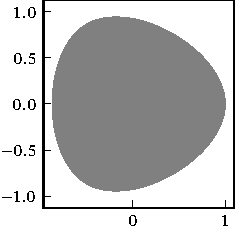
\includegraphics{figures/convex.pdf}
    \caption{\(\numset{R}^2\)の凸集合.}
  \end{minipage}%
  \begin{minipage}{0.5\linewidth}
    \centering
    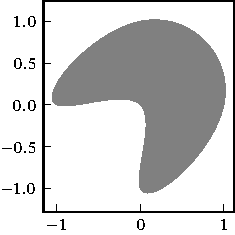
\includegraphics{figures/non_convex.pdf}
    \caption{\(\numset{R}^2\)の凸集合でない部分集合.}
  \end{minipage}
\end{figure}

\begin{theorem}{凸射影定理}{convex_projection_theorem}\index{とつしゃえいていり@凸射影定理}\index{しゃえいていり@射影定理!とつ@凸\texttwoemdash}
  \(H\)をヒルベルト空間とする.また,\(x\in H\)かつ,集合\(C\subset H\)は空でない閉凸集合とする.
  このとき,\(\argmin_{y\in C}\vnorm{x-y}\)はただ1つの元からなる集合である.
\end{theorem}

\begin{proof}
  まず,\(\argmin_{y\in C}\vnorm{x-y}\)が空でないことを示す.\(\delta=\inf\Set{\vnorm{x-y}\given y\in C}\)とおくと,
  集合\(A_n=\Set{y\in C\given\vnorm{x-y}\leq\delta+1/n}\)(\(n=1,2,\dotsc\))は\(n\)の値によらず空でない.
  そこで,\(C\)上の点列\(\seq{a_n}\)を各\(n\)に対して\(a_n\in A_n\)となるようにとれる.
  \(0\leq\vnorm{x-a_n}-\delta\leq 1/n\to 0\)(\(n\to\infty\))なので,\(\seq{a_n}\)がある点\(x_{\mathord{\ast}}\)に収束すれば,\nameref{proposition:norm_continuous}より
  \(\vnorm{x-x_{\mathord{\ast}}}=\lim_{n\to\infty}\vnorm{x-a_n}=\delta\)である.さらに,\(C\)は閉集合だから\(x_{\mathord{\ast}}\in C\),よって\(x_{\mathord{\ast}}\in\argmin_{y\in C}\vnorm{x-y}\)である.

  つまり,\(\seq{a_n}\)の極限点\(x_{\mathord{\ast}}\)が存在すること,すなわち,\(\seq{a_n}\)がコーシー列であることを示せばよい.
  \(m,n\in\numset{N}\)を任意にとる.\nameref{theorem:median_theorem}より
  \begin{gather*}
    \vnorm{(a_m-x)+(a_n-x)}^2+\vnorm{a_m-a_n}^2 = 2(\vnorm{a_m-x}^2+\vnorm{a_n-x}^2), \\
    \vnorm{a_m-a_n}^2 = 2\vnorm{x-a_m}^2+2\vnorm{x-a_n}^2-4\vnorm*{x-\frac{a_m+a_n}{2}}^2
  \end{gather*}
  である.\(a_m\in A_m\),\(a_n\in A_n\)かつ,\(C\)は凸集合だから\((a_m+a_n)/2\in C\)で
  \[
    \vnorm{a_m-a_n}^2 \leq 2\pqty*{\delta+\frac{1}{m}}^2+2\pqty*{\delta+\frac{1}{n}}^2-4\delta^2
    \to 0\quad(m,n\to\infty)
  \]
  である.よって\(\seq{a_n}\)はコーシー列だから,\(\argmin_{y\in C}\vnorm{x-y}\)は空でない.

  次に,\(\argmin_{y\in C}\vnorm{x-y}\)の元は1つしかないことを示す.\(x_{\mathord{\ast}},x'_{\mathord{\ast}}\in\argmin_{y\in C}\vnorm{x-y}\)とする.
  このとき\(\vnorm{x-x_{\mathord{\ast}}}=\vnorm{x-x'_{\mathord{\ast}}}=\delta\),\((x_{\mathord{\ast}}+x'_{\mathord{\ast}})/2\in C\)なので\(\vnorm{x_{\mathord{\ast}}-x'_{\mathord{\ast}}}^2=2\delta^2+2\delta^2-4\vnorm{x-(x_{\mathord{\ast}}+x'_{\mathord{\ast}})/2}^2\leq 0\),したがって\(x_{\mathord{\ast}}=x'_{\mathord{\ast}}\)である.
\end{proof}

\begin{theorem}{射影定理}{projection_theorem}\index{しゃえいていり@射影定理}
  \(H\)をヒルベルト空間とする.また,\(x\in H\)かつ,\(V\)は\(H\)の閉部分空間とする.
  このとき,\(V\)の元\(m\)に関する以下の条件は同値であり,条件を満たす\(m\)はただ1つ存在する.
  \begin{enumerate}
    \item \(m\in\argmin_{y\in V}\vnorm{x-y}\)である.
    \item 任意の\(v\in V\)に対して\(\innerp{x-m}{v}=0\)である.
  \end{enumerate}
\end{theorem}

\begin{proof}
  閉部分空間は閉凸集合だから,\nameref{theorem:convex_projection_theorem}より\(n\in\argmin_{y\in V}\vnorm{x-y}\)を満たす\(n\)が一意に定まる.
  あとはp.\pageref{xr-proposition:finite_projection}の\cref{xr-proposition:finite_projection}と同様に示せる.
\end{proof}

\begin{definition}{直交射影}{hilbert_projection}\index{ちょっこうしゃえい@直交射影}\index{proj@\(\proj_Vx\)}
  \cref{theorem:projection_theorem}の\(m\)を\(x\)の\(V\)への\termdef{直交射影}(orthogonal projection)といい,\(\proj_Vx\)と表す.
\end{definition}

\begin{proposition}{}{orthogonal_direct_sum}
  \(H\)はヒルベルト空間で,\(V\)は\(H\)の閉部分空間とする.このとき\(H=V\oplus\pcomp[H]{V}\)である.
\end{proposition}

\subsection{正規直交系}

\nameref{theorem:projection_theorem}は直交射影\(\proj_Vx\)の存在を示す定理であり,具体的な式を与えるものではない.
しかし,\(V\)が正規直交系によって生成される空間(正確にはその閉包)であれば,\(\proj_Vx\)の具体的な式が得られる.

\begin{definition}{正規直交系}{ons}\index{せいきちょっこうけい@正規直交系}
  \(H\)をヒルベルト空間,\(\seq{\phi_n}\)を\(H\)上の点列とする.\(\innerp{\phi_i}{\phi_j}=\kdelta{i}{j}\)(\(i,j\in\numset{N}\))であるとき,\(\seq{\phi_n}\)は\termdef{正規直交系}(orthonormal system; ONS)であるという.
\end{definition}

\begin{theorem}{ベッセルの不等式}{bessels_inequality}\index{べっせるのふとうしき@ベッセルの不等式}
  \(H\)をヒルベルト空間とする.\(H\)上の点列\(\seq{\phi_n}\)が正規直交系なら,任意の\(x\in H\)に対して次式が成立する.
  これを\termdef{ベッセルの不等式}(Bessel's inequality)という.
  \begin{equation}
    \label{equation:bessels_inequality}
    \sum_{n=1}^\infty\abs{\innerp{x}{\phi_n}}^2 \leq \vnorm{x}^2
  \end{equation}
\end{theorem}

\begin{proof}
  p.\pageref{xr-equation:pre_bessels_inequality}の\cref{xr-equation:pre_bessels_inequality}と同様に計算すると,
  任意の\(z_1,\dots,z_m\in\numset{C}\)に対して次式が成り立つと分かる.
  \[
    \vnorm*{x-\sum_{k=1}^mz_k\phi_k}^2 = \vnorm{x}^2+\sum_{k=1}^m\abs{z_k-\innerp{x}{\phi_k}}^2-\sum_{k=1}^m\abs{\innerp{x}{\phi_k}}^2
  \]

  したがって,特に\(z_k=\innerp{x}{\phi_k}\)なら
  \[
    \vnorm{x}^2 = \vnorm*{x-\sum_{k=1}^m\innerp{x}{\phi_k}\phi_k}^2+\sum_{k=1}^m\abs{\innerp{x}{\phi_k}}^2
    \geq \sum_{k=1}^m\abs{\innerp{x}{\phi_k}}^2
  \]
  である.よって,級数\(\sum\abs{\innerp{x}{\phi_n}}^2\)は上に有界な正項級数だから収束し,級数の和は\cref{equation:bessels_inequality}を満たす.
\end{proof}

\cref{theorem:bessels_inequality}の状況で,点列\(\seq{x_n}\)を\(x_n=\sum_{k=1}^n\innerp{x}{\phi_k}\phi_k\)で定義すると,
\(\seq{x_n}\)は収束列になる.実際,\(m>n\)なら
\[
  \vnorm{x_m-x_n}^2 = \vnorm*{\sum_{k=n+1}^m\innerp{x}{\phi_k}\phi_k}^2
  = \sum_{k=n+1}^m\abs{\innerp{x}{\phi_k}}^2
\]
となるので,\(\seq{x_n}\)がコーシー列であることと,級数\(\sum\abs{\innerp{x}{\phi_n}}^2\)がコーシー列であることとは同値である.
そして,\cref{equation:bessels_inequality}の級数は収束しているから,\(\seq{x_n}\)はコーシー列である.

\begin{proposition}{}{orthonormal_system_and_projection}
  \(H\)をヒルベルト空間とする.\(H\)上の点列\(\seq{\phi_n}\)が正規直交系なら,任意の\(x\in H\)について次式が成立する.
  \[
    \proj_{\clsr V}x = \sum_{n=1}^\infty\innerp{x}{\phi_n}\phi_n
    \quad(V=\spannedby\Set{\phi_1,\phi_2,\dotsc})
  \]
\end{proposition}

\begin{proof}
  \(v\in\clsr V\)を任意にとる.閉包の定義から,\(V\)上の点列\(\seq{v_n}\)で\(v_n\to v\)(\(n\to\infty\))を満たすものがある.
  \(V=\bigcup_{n=1}^\infty\spannedby\basis{B}_n\)(\(\basis{B}_n=\Set{\phi_1,\dots,\phi_n}\))なので,\(n\)の値に応じて\(v_n\in\spannedby\basis{B}_{d_n}\)を満たす\(d_n\in\numset{N}\)をとれて,
  \(v_n\)は\(\basis{B}_{d_n}\)の元の線型結合で\(v_n=\sum_{j=1}^{d_n}\midx{z}{n}{j}\phi_j=\midx{z}{n}{1}\phi_1+\dots+\midx{z}{n}{d_n}\phi_{d_n}\)とおける.

  \(p=\sum_{i=1}^\infty\innerp{x}{\phi_i}\phi_i\)とする.\nameref{proposition:inner_products_continuous}と\(\innerp{\phi_i}{\phi_j}=\kdelta{i}{j}\)より
  \begin{gather*}
    \innerp{x-p}{\phi_j} = \innerp*{x-\sum_{i=1}^\infty\innerp{x}{\phi_i}\phi_i}{\phi_j}
    = \innerp{x}{\phi_j}-\sum_{i=1}^\infty\innerp{x}{\phi_i}\innerp{\phi_i}{\phi_j}
    = 0, \\
    \innerp{x-p}{v} = \innerp*{x-p}{\lim_{n\to\infty}\sum_{j=1}^{d_n}\midx{z}{n}{j}\phi_j}
    = \lim_{n\to\infty}\sum_{j=1}^{d_n}\midx{\conj{z}}{n}{j}\innerp{x-p}{\phi_j}
    = 0
  \end{gather*}
  である.また,\(\clsr V\)の定義から\(\clsr V\)は\(H\)の閉部分空間であることがしたがう.
  よって,\nameref{theorem:projection_theorem}より\(p=\proj_{\clsr V}x\)である.
\end{proof}

\cref{proposition:orthonormal_system_and_projection}より,\(\clsr V=H\)であれば任意の\(x\in H\)に対して
\[
  x = \proj_Hx
  = \sum_{n=1}^\infty\innerp{x}{\phi_n}\phi_n
\]
が成立する.そのような正規直交系\(\seq{\phi_n}\)は完全正規直交系と呼ばれる.

\begin{definition}{完全正規直交系}{cons}\index{かんぜんせいきちょっこうけい@完全正規直交系}\index{せいきちょっこうけい@正規直交系!かんぜん@完全\texttwoemdash}\index{CONS|see{完全正規直交系}}
  \(H\)をヒルベルト空間,\(\seq{\phi_n}\)を\(H\)上の正規直交系とする.\(\spannedby\Set{\phi_1,\phi_2,\dotsc}\)が\(H\)において稠密であるとき,\(\seq{\phi_n}\)は\termdef{完全正規直交系}(complete orthonormal system; CONS)であるという.
\end{definition}

\section{\texorpdfstring{\(\Lebesgue{p}\)}{Lp}空間}
\label{section:lp_space}

\begin{definition}{\(\Lebesgue{p}\)空間}{Lp_space}\index{Lpkukan@\(\Lebesgue{p}\)空間}
  集合\(\Omega\subset\numset{R}\)はルベーグ可測とする.各\(p\in\coival{1}{+\infty}\)に対し,可測関数\(f\colon\Omega\to\numset{K}\)で
  \[
    \Lpnorm{p}{f} = \pqty*{\int_\Omega\abs{f(t)}^p\intd{t}}^{1/p}
  \]
  の値が有限であるものの全体集合を\(\Lebesgue{p}(\Omega)\)とおく.このとき,ほとんどいたるところ等しい関数を同一視すれば,\(\Lebesgue{p}(\Omega)\)は\(\Lpnorm{p}{\holder}\)をノルムとしてバナッハ空間になる.
  このバナッハ空間を\termdef{\(\Lebesgue{p}\)空間}(\(\Lebesgue{p}\) space)という.
\end{definition}

\begin{proposition}{\(\Lebesgue{2}\)空間の性質}{L2_space_property}
  \(p=2\)のときのみ\(\Lebesgue{p}(\Omega)\)はヒルベルト空間になり,内積は次の式で表される.
  \[
    \innerp{f}{g} = \int_\Omega f(t)\conj*{g(t)}\intd{t}\quad(f,g\in\Lebesgue{2}(\Omega))
  \]
\end{proposition}

\section{フーリエ級数展開}

\(\torus=\ccival{-\krez}{\krez}\)とする.

\begin{theorem}{リース・フィッシャーの定理}{riesz_fischer}\index{りーすふぃっしゃーのていり@リース・フィッシャーの定理}
  \(\Lebesgue{2}(\torus)\)上の関数列\(\seq{\phi_n}_{n\in\numset{Z}}\)を
  \[
    \phi_n(t) = \frac{\napr^{\iuni nt}}{\sqrt{2\krez}}
  \]
  で定義する.このとき\(\seq{\phi_n}_{n\in\numset{Z}}\)は完全正規直交系である.これを\termdef{リース・フィッシャーの定理}(Riesz–Fischer theorem)という.
\end{theorem}

\nameref{theorem:riesz_fischer}によれば
\[
  \hat{f}_n = \frac{\innerp{f}{\phi_n}}{\sqrt{2\krez}}
  = \frac{1}{2\krez}\int_{\torus}f(t)\napr^{-\iuni nt}\intd{t}\quad(n\in\numset{Z})
\]
とおくと,\(\torus\)上の関数列\(S_N(t)=\sum_{n=-N}^N\hat{f}_n\napr^{\iuni nt}\)は\(f\)に\(\Lebesgue{2}\)収束する.このことを形式的に
\[
  f(t) = \sqlim_{N\to\infty}\sum_{n=-N}^N\hat{f}_n\napr^{\iuni nt}\quad(t\in\torus)
\]
と表そう\index{lim@\(\sqlim\)}\footnote{\(\sqlim\)はlimit in the mean(平均収束)の略.}.

\begin{definition}{フーリエ級数展開}{fourier_series_expansion}\index{ふーりえきゅうすうてんかい@フーリエ級数展開}
  各\(f\in\Lebesgue{2}(\torus)\)に対して,次式を\(f\)の\termdef{フーリエ級数展開}(Fourier series expansion)という.
  \[
    f(t) = \sqlim_{N\to\infty}\sum_{n=-N}^N\hat{f}_n\napr^{\iuni nt}\quad(t\in\torus)
  \]
\end{definition}

\begin{note}
  \cref{definition:fourier_series_expansion}で「形式的に」と断りを入れたのは,\(f(t)=\sqlim_{N\to\infty}S_N(t)\)(\(t\in\torus\))であっても,
  各\(a\in\torus\)に対して数列\(\seq{S_N(a)}\)が\(f(a)\)に収束するとは言えないからである.あくまで\(\sqlim\)は,関数列の\(\Lebesgue{2}\)収束
  \[
    f(t)=\sqlim_{N\to\infty}S_N(t)\quad(t\in\torus)
    \iff\lim_{N\to\infty}\int_{\torus}\abs{f(t)-S_N(t)}^2\intd{t} = 0
  \]
  で定義される.
\end{note}

\section{多重解像度解析}

\begin{definition}{多重解像度解析}{multiresolution_analysis}\index{たじゅうかいぞうどかいせき@多重解像度解析}\index{MRA|see{多重解像度解析}}
  \(\Lebesgue{2}(\numset{R})\)の閉部分空間の列\(\seq{V_n}_{n\in\numset{Z}}\)が以下の条件を満たすとき,
  \(\seq{V_n}_{n\in\numset{Z}}\)は\termdef{多重解像度解析}(multiresolution analysis; MRA)をなすという.
  \begin{enumerate}
    \item \(\dotsb\subset V_{-1}\subset V_0\subset V_1\subset\dotsb\)
    \item \(\bigcap_{n\in\numset{Z}}V_n=\Set{0}\),\(\clsr(\bigcup_{n\in\numset{Z}}V_n)=\Lebesgue{2}(\numset{R})\)
    \item \(f(\holder)\in V_n\iff f(2\holder)\in V_{n+1}\),ただし\(n\)は任意の整数.
    \item \(\seq{\phi(\holder-n)}_{n\in\numset{Z}}\)が\(V_0\)の完全正規直交系となる\(\phi\in V_0\)が存在する.
  \end{enumerate}
\end{definition}

\begin{figure}[htbp]
  \begin{minipage}{0.5\linewidth}
    \centering
    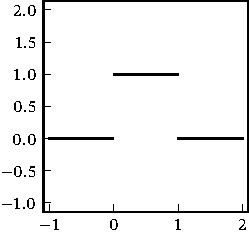
\includegraphics{figures/haar_scaling}
    \caption{Haarのスケーリング関数.}
  \end{minipage}%
  \begin{minipage}{0.5\linewidth}
    \centering
    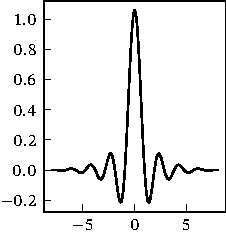
\includegraphics{figures/meyer_scaling}
    \caption{Meyerのスケーリング関数.}
  \end{minipage}
\end{figure}

\section*{演習問題}
\addcontentsline{toc}{section}{演習問題}

\end{document}
